\documentclass[a4paper,9pt]{article} 
\usepackage{extsizes} % Возможность сделать 9-й шрифт(иначе минимально 12 вроде)
\usepackage{geometry} % Простой способ задавать поля
    \geometry{top=15mm}
    \geometry{bottom=15mm}
    \geometry{left=15mm}
    \geometry{right=15mm}
    \geometry{headsep=1.5mm}
    \geometry{head=5mm}

%%% Работа с русским языком
\usepackage{cmap}                   % поиск в PDF
\usepackage{mathtext}               % русские буквы в формулах
\usepackage[T2A]{fontenc}           % кодировка
\usepackage[utf8]{inputenc}         % кодировка исходного текста
\usepackage[english,russian]{babel} % локализация и переносы

%%% Дополнительная работа с математикой
\usepackage{amsmath,amsfonts,amssymb,amsthm,mathtools} % AMS
\usepackage{icomma} % "Умная" запятая: $0,2$ --- число, $0, 2$ --- перечисление

\usepackage{graphicx} % работа с картинками

%% Номера формул
\mathtoolsset{showonlyrefs=true} % Показывать номера только у тех формул, на которые есть \eqref{} в тексте.

\usepackage{wrapfig} % Обтекание рисунков и таблиц текстом


%% Шрифты
\usepackage{euscript} % Шрифт Евклид
\usepackage{mathrsfs} % Красивый матшрифт

\usepackage{multicol} % Для создания нескольких колонок

\usepackage{fancyhdr} % Колонтитулы
    \pagestyle{fancy}
    \fancyhf{} % очистка текущих значений
    \renewcommand{\headrulewidth}{0mm}  % Толщина линейки, отчеркивающей верхний колонтитул. renewcommand - переназначение команды
    
%% TkiZ
\usepackage{tikz}  
\usetikzlibrary{positioning, graphs}
\documentclass{article}

\begin{document}
    \begin{center}
    \large
    \Huge \textbf{Федеральное государственное автономное образовательное учреждение высшего образования} \\
    \Huge «Университет ИТМО»\\
    \vspace{2cm}
    Дисциплина: Информатика \\ 
    \vspace{5cm}
    Лабораторная работа №7 \\
    Работа с системой компьютерной вёрстки \TeX \vspace{8cm}
\end{center}
\begin{flushright}
    \LARGE \textbf{Выполнил:} Кривоносов Егор Дмитриевич \\
    \LARGE \textbf{Группа:} Р3111 \\
    \LARGE \textbf{Преподаватель:} Балакшин Павел Валерьевич \\
\end{flushright}
\vfill
\begin{center}
    \LARGE Санкт-Петербург \\ 
    \LARGE 2019 г.
\end{center}
    \setcounter{page}{56} % начать нумерацию страниц с 56
\newpage
\setlength{\columnsep}{1cm} % расстояние между столбцами текста
\begin{multicols}{2} % разделить структуру страницы на две колонки
\fancyhf{}
\chead{\footnotesize
О Т В Е Т Ы , У К А З А Н И Я , Р Е Ш Е Н И Я}
\rhead{\thepage}
\begin{wrapfigure}{l}{0.5\linewidth}
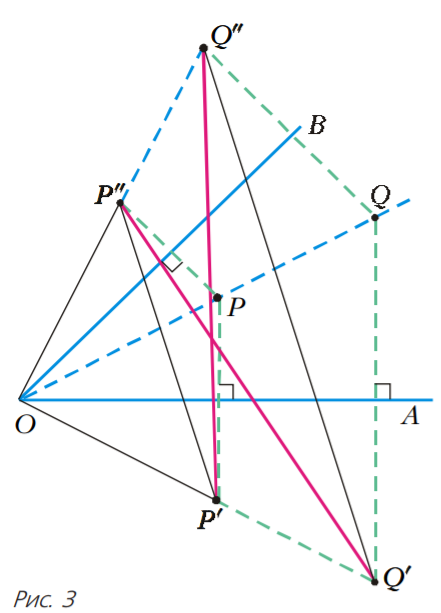
\includegraphics[scale=0.5]{img1.png}
\end{wrapfigure}
    \noindent
    Обратим внимание, что по условию первыми «стреляли» бактерии, причем произвели они не менее \emph{двух} «залпов». Так что рассмотренный сейчас момент (когда имеется 9\emph{М} бактерий и 31\emph{М} вирусов) вполне мог бы быть исходным. В этом случае общее количество микробов равно 9\emph{М} + 31\emph{М} = 40\emph{М}, а так как по условию это число равно 2000, то \emph{М} = 2000/40 = 50. Таким образом, в данном случае в итоге борьбы осталось в живых 50 бактерий и 50 вирусов. Предположение, что этот обмен любезностями продолжался дольше, приводит к противоречию. Рассмотрев аналогично вторую возможность, когда последний удар нанесли вирусы, опять получаем противоречие с условием. \\ 
    Итак, ответ: в результате разразившегося побоища в живых осталось по 50 бактерий и вирусов.
    \begin{center}
        \large
        \emph{Задачи}\\
    \end{center}
    \begin{center}
        \emph{(см. «Квант» №5)}
    \end{center}
    \textbf{1.} Слагаемых ШАХ меньше 10, иначе их сумма была бы четырехзначной. Запишем ребус в виде $ШАХ \times У = МАТ$, где У – неизвестная отличная от 0 цифра, возможно совпадающая с одной из цифр, зашифрованных буквами Ш, А, Х, М, Т. Цифры Ш = 1, А = 3, Х = 4, М = 9, Т = 8 удовлетворяют ребусу: $134 \times 7 = 938$. Покажем, что значение У = 7 наибольшее. \\ 
    Предположим, что У = 8 или У = 9. Поскольку в этом случае наименьшим трехзначным числом, представленным словом ШАХ, является число 123 (так как $Ш = 1, А \neq 0, Х \neq 0$), то значение У = 9 не подходит: $123 \times 9 = 1107$. Легко проверить, что в случае У = 8 и наименьшем значении А = 2 ребус $12Х \times 8 = 92Т$ для букв Х и Т решений не имеет, в случае же $А \geq 3$ произведение $1АХ \times 8$ получается четырехзначным. Итак, гроссмейстер объявил шах семь раз. \\ 
    \textbf{2.} Пусть первая программа содержала \emph{K} клипов. Тогда, по условию, вторая программа содержала 1,5\emph{K} клипов, а Бивису понравились \emph{K}/5 клипов первой программы и (1,5\emph{K}) : 2 = 3\emph{K}/4 клипов второй программы. По смыслу задачи все эти числа должны быть целыми, откуда следует, что \emph{K} делится на 4 и на 5, т.е. на 20. Итак, \emph{K} = 20\emph{m}, где \emph{m} – натуральное число. Тогда вторая программа содержала $1,5 \times 20m = 30m$ клипов, а третья программа – все остальные, т.е. $200 - 20m - 30m = 200 - 50m$ клипов. Это число должно быть положительным, в связи с чем $200 - 50m > 0$, откуда $m < 4$. Далее, Бивису понравились всего  $(20m/5) + (30m/2) = 19m$ клипов. Батт-Хеду понравилось столько же клипов, причем в это число входили все клипы третьей программы. Поэтому $19m \geq 200 - 50m$, и $m \geq 200/69 > 2,8$.\\ 
    Таким образом, $2,8 < m < 4$. Единственное натуральное число, удовлетворяющее этим условиям, это \emph{m} = 3. Этот результат позволяет нам восстановить всю картину. Итак, первая программа содержала $20 \times 3 = 60$ клипов, вторая – $1,5 \times 60 =  90$ клипов, третья $200 - 60 - 90 = 50$ клипов. Бивису понравились $(60/5) + (90/2) = 57$ клипов, Батт-Хеду – столько же. Ну, а не понравилось каждому из них $200 - 57 = 143$ клипа. \\ 
    \textbf{3.} Сомкнем выходящие из города дороги в еще один перекресток. Пусть \emph{N} – общее количество перекрестков вместе с этим. Так как в каждом из перекрестков сходится по три дороги, то общее количество оконечностей дорог 3\emph{N}. Это число четное, поскольку каждая дорога в нашем случае имеет два конца. Следовательно, число \emph{N} – четное, и в городе имеется нечетное количество перекрестков. Поскольку в каждом из них сходятся по одной дороге трех разных цветов, то для каждого цвета найдется дорога, не имеющая двух оконечностей в городе. Итак, все три выходящие из города дороги непременно имеют разные цвета.\\ 
    \textbf{4.} Воспользуемся следующим очевидным утверждением. Имеется \emph{K} карточек. Известно, что какие бы \emph{M} из них ни взять, среди них окажется не менее \emph{N} особых. В этом случае среди \emph{K} карточек имеется не менее $K - M + N$ особых. Считая, что особые карточки – синие, в приложении к условию задачи имеем:\\
    \begin{center}
        \begin{tabular}{|c|c|c|c|}
            \hline
            \emph{K} & \emph{M} & \emph{N} & \emph{K - M + N} \\ \hline
            100 & 80 & 20 & 40 \\ \hline
            40 & 10 & 2 & 32 \\ 
            \hline
        \end{tabular}
    \end{center}
    Считая, что особые карточки – красные, в приложении к условию задачи имеем: \\
    \begin{center}
        \begin{tabular}{|c|c|c|c|}
            \hline
            \emph{K} & \emph{M} & \emph{N} & \emph{K - M + N} \\ 
            \hline
            100 & 50 & 30 & 80 \\ \hline
            80 & 20 & 10 & 70 \\ \hline
            70 & 5 & 3 & 68 \\ 
            \hline
        \end{tabular}
    \end{center}
    Итак, в колоде находятся 32 синих и 68 красных карточек.\\ 
    \textbf{5.} Нет, не удастся. Если бы существовало разбиение пятиугольного поля на параллелограммы, то можно было бы пройти от любого края поля к другому краю, двигаясь по цепочке параллелограммов. Поскольку в пятиугольнике не для каждой стороны существует параллельная ей сторона, то этого сделать нельзя.
    \begin{center}
        \textbf{Кеплер и винные бочки – австрийские и рейнские}
    \end{center}
    \textbf{1.} Учитывая, что AB = OA/\emph{sin a}, имеем \[E = \frac{C}{OA^2} \sin^2 \alpha \cos^2 \alpha . \]  Таким образом, если лампу поместить в вершину конуса максимального объема, то окружность его основания получит наибольшую освещенность.\\  
    \textbf{2.} Обозначим $a = 4 - x$, тогда $b = 4 + x$ и $ab(b - a) = ax(16 - x^2)$, причем $0\leq x \leq 4$. Максимум достигается при $x = 4/\sqrt{3}$ и равен $256/(3\sqrt{3})$. \\ 
    \textbf{3.} Обозначим буквой \emph{R} радиус шара, а буквами \emph{r} и \emph{h} – радиус и высоту конуса. Тогда объем конуса равен $V = \pi r^2h/3$.Продолжив высоту конуса до пересечения с шаром, получим отрезок длиной $2R - h$. Таким образом, через одну точку (центр основания конуса) проходят две хорды: одна из них состоит из отрезков длиной \emph{h} и $2R - h$, а другая – из двух отрезков длиной \emph{r} каждый. Значит, $r^2 = h(2R - h)$, так что $V = \pi h^2(2R - h)/3$. Применяя неравенство о среднем арифметическом и среднем геометрическом, получим \[\frac{3V}{4\pi} = \frac{h}{2}\cdot\frac{h}{2}\cdot(2R - h)\leq\left(\frac{\dfrac{h}{2} + \dfrac{h}{2} + 2R - h}{3}\right)^3 = \frac{8}{27}R^3,\] где равенство достигается при $\dfrac{h}{2} = 2R - h$, т.е. при $h = \dfrac{4}{3}R$.
\end{multicols}
    \begin{center}
    \noindent
    Используя TkiZ:\\
    \vspace{2mm}
\end{center}

\begin{tikzpicture}
\tikzstyle{roundnode} = [circle, draw=black, thick, minimum size=1.5cm]
\tikzstyle{edge} = [->, thick, auto]

% Создвание кругов
\node[roundnode] (b1) {b1};
\node[roundnode] (b2) [right =5cm of b1] {b2};
\node[roundnode] (b3) [right =5cm of b2] {b3};
\node[roundnode] (b4) [below =5cm of b1] {b4};
\node[roundnode] (b5) [below =5cm of b2] {b5};
\node[roundnode] (b6) [below =5cm of b3] {b6};

% Создание векторов перехода
\draw[edge]  (b1) -- node {$z_3$} (b2);
\draw[edge]  (b3) -- node [above] {$z_2$} (b2);
\draw[edge]  (b6) -- node {$z_3$} (b3);
\draw[edge]  (b2) -- node [near start] {$z_1$} (b6);
\draw[edge]  (b5) -- node [near start] {$z_3$} (b3);
\draw[edge]  (b1) -- node {$z_2$} (b5);
\draw[edge]  (b5) -- node {$z_2$} (b4);
\draw[edge]  (b4) -- node {$z_1$} (b1);

% Создание изогнутых линий
\path [->] (b1) edge [loop left] node {$z_1$}(b1); 
\path [->] (b2) edge [loop above] node {$z_2$}(b2); 
\path [->] (b4) edge [loop left] node {$z_3$}(b4); 
\path [->] (b3) edge [bend left] node [auto] {$z_1$}(b6); 
\path [->] (b6) edge [bend left] node [auto] {$z_2$}(b4); 

\end{tikzpicture}
    \vspace{5cm}
    \usetikzlibrary{arrows}
\pagestyle{empty}
\begin{document}
\begin{center}
    \noindent
    Созданный с помощью Geogebra:

\begin{tikzpicture}[line cap=round,line join=round,>=triangle 45,x=1cm,y=1cm]

\draw (-4.5,-3.5) rectangle (4.5,3);
\draw [line width=0.5pt] (2.9708949242827054,-1.4470035613714107) circle (0.5687031205152061cm);
\draw [line width=0.5pt] (2.970894924282706,1.4178984856541166) circle (0.5687031205152331cm);
\draw [line width=0.5pt] (0,-1.4033459477954695) circle (0.568703120515207cm);
\draw [line width=0.5pt] (-0.014552537858647102,1.4178984856541166) circle (0.5687031205152336cm);
\draw [line width=0.5pt] (-3,1.4324510235127637) circle (0.5687031205152334cm);
\draw [line width=0.5pt] (-2.986664196004032,-1.3980664321823293) circle (0.5687031205152326cm);

\draw [->,line width=0.1pt] (-2.4315268473218885,1.448622417020211) -- (-0.5827129394473904,1.4427379170139971);
\draw [->,line width=0.1pt] (2.4024039088770754,1.4334292514703608) -- (0.5539799587817273,1.4318282935360354);
\draw [->,line width=0.1pt] (0.3735270838599657,1.0021853075005935) -- (2.6224007236130737,-0.9975872383663738);
\draw [->,line width=0.1pt] (0.39229483108621066,-0.991608161350291) -- (2.567903158183671,1.0166244200329453);
\draw [->,line width=0.1pt] (2.9931126707395,-0.8787346012599907) -- (2.9915469281428897,0.8495704694343259);
\draw [->,line width=0.1pt] (-3.0058922975493934,-0.8296884598833278) -- (-3.004666132735822,0.8637670458159625);
\draw [->,line width=0.1pt] (-2.616267564247627,1.012721757157277) -- (-0.3634898625164298,-0.9659692690258752);
\draw [->,line width=0.1pt] (-0.5686423133586304,-1.3950297742836089) -- (-2.4180158195747135,-1.390175724478738);

\draw [<-, shift={(2.3967395313364595,0.126754489390692)},line width=0.1pt]  plot[domain=-0.8603882048439315:0.7863479730960713,variable=\t]({1*1.608263296528255*cos(\t r)+0*1.608263296528255*sin(\t r)},{0*1.608263296528255*cos(\t r)+1*1.608263296528255*sin(\t r)});
\draw [<-, shift={(-0.05337578460024872,2.1105180961775076)},line width=0.1pt]  plot[domain=4.131218338684883:5.297807224399998,variable=\t]({1*4.760402030350322*cos(\t r)+0*4.760402030350322*sin(\t r)},{0*4.760402030350322*cos(\t r)+1*4.760402030350322*sin(\t r)});
\draw [<-, shift={(-3.7719801814250915,1.4369936551945872)},line width=0.1pt]  plot[domain=0.4110144652240396:5.832176174009245,variable=\t]({1*0.2362826572245055*cos(\t r)+0*0.2362826572245055*sin(\t r)},{0*0.2362826572245055*cos(\t r)+1*0.2362826572245055*sin(\t r)});
\draw [<-, shift={(-3.770945616120117,-1.3795850640439742)},line width=0.1pt]  plot[domain=0.41101446522403806:5.832176174009247,variable=\t]({1*0.23628265722450625*cos(\t r)+0*0.23628265722450625*sin(\t r)},{0*0.23628265722450625*cos(\t r)+1*0.23628265722450625*sin(\t r)});
\draw [<-, shift={(-0.016668102767723764,2.1623099343841052)},line width=0.1pt]  plot[domain=-1.0745935833821765:4.2218700808118665,variable=\t]({1*0.20939539267107515*cos(\t r)+0*0.20939539267107515*sin(\t r)},{0*0.20939539267107515*cos(\t r)+1*0.20939539267107515*sin(\t r)});

\begin{scriptsize}
\draw[color=black] (-2.9866641960040314,1.4524800977696472) node {$b_1$};
\draw[color=black] (0.011158602877274187,1.4524800977696472) node {$b_2$};
\draw[color=black] (2.9980864774758747,1.4524800977696472) node {$b_3$};
\draw[color=black] (-2.94487434743862,-1.395817322525182) node {$b_4$};
\draw[color=black] (0.011158602877274187,-1.395817322525182) node {$b_5$};
\draw[color=black] (2.994428863899933,-1.395817322525182) node {$b_6$};
\draw[color=black] (4.245947119743585,0.02267377404629129) node {$z_1$};
\draw[color=black] (1.0443887908412195,0.8503006669786457) node {$z_1$};
\draw[color=black] (-3.306820028894268,0.02267377404629129) node {$z_1$};
\draw[color=black] (-4.238182451847684,1.5342699463350589) node {$z_1$};
\draw[color=black] (0.025711140735921303,-2.8859660326725967) node {$z_2$};
\draw[color=black] (1.6992529944803396,1.8398732413666476) node {$z_2$};
\draw[color=black] (-1.4149901072701432,0.4282770690778801) node {$z_2$};
\draw[color=black] (-1.4295426451287903,-1.5926579282635355) node {$z_2$};
\draw[color=black] (-0.017946472840020045,2.5130255128854732) node {$z_2$};
\draw[color=black] (-1.5023053344220259,1.8544257792252947) node {$z_3$};
\draw[color=black] (0.6369177307991002,-0.22658713456123883) node {$z_3$};
\draw[color=black] (2.7470357203029323,0.02267377404629129) node {$z_3$};
\draw[color=black] (-4.223629913989036,-1.1870546332319467) node {$z_3$};

\end{scriptsize}
\end{tikzpicture}
\end{center}
\end{document}

\end{document}\documentclass[a4paper,9pt]{article} 
